\documentclass{article}
\usepackage[utf8]{inputenc}
\usepackage{amssymb}
\usepackage{comment}
\usepackage{graphicx}
\usepackage{amsmath,amsfonts,amssymb,amsthm}
\usepackage{mathtools}
\usepackage{commath}

\title{Homework 2}
\author{Vladimir Frants, Yunhua Zhao, Mohamed Ben Zid}
\date{September 2020}

\begin{document}

\maketitle

\section{Exercise 2.6}

\subsection{a)}

$\mathcal{O}$


From \emph{1.7} the point $\theta^{*}$ we have: 

$$\frac{\sin(\alpha_{1}(\theta^{*}))}{\sin(\alpha_{2}(\theta^{*}))} = \frac{v_1}{v_2}$$

Multiply both sides by $\sin(\alpha_{2}(\theta^{*}))$:

$$\sin(\alpha_{1}(\theta^{*}))=\frac{v_{1}\cdot \sin(\alpha(\theta^{*}))}{v_{2}}$$

Divide both sides by $v_{1}$:

$$\frac{\sin(\alpha_{1}(\theta^{*}))}{v_{1}}=\frac{\sin(\alpha_{2}(\theta^{*}))}{v_{2}}$$

$$\frac{\sin(\alpha_{1}(\theta^{*}))}{v_{1}} - \frac{\sin(\alpha_{2}(\theta^{*}))}{v_{2}} = 0$$

So: 

$$J'(\theta)= \frac{\sin(\alpha_{1}(\theta))}{v_{1}} - \frac{\sin(\alpha_{2}(\theta))}{v_{2}}$$

Therefore:

$$\theta_{n+1} = \theta_{n} - \epsilon(\frac{\sin(\alpha_{1}(\theta_{n}))}{v_{1}} - \frac{\sin(\alpha_{2}(\theta_{n}))}{v_{2}})$$

Here we have a vector field: 

$$G(\theta) = \frac{\sin(\alpha_{2}(\theta))}{v_{2}} - \frac{\sin(\alpha_{1}(\theta))}{v_{1}}$$

A function $G(\theta)$ is Lipschitz-continuous on $\theta\in(-\infty, \infty)$ because it is differentiable at $x\in{(-\infty, \infty)}$ for $v_1 \neq 0, v_2 \neq 0$. 

So we have Lipschitz continuous function $G:\mathbb{R}\rightarrow\mathbb{R}$, and recurison of form:

$$\theta_{n+1}+\epsilon(G(\theta_{n}) + \beta_{\epsilon}(\theta_n)), n\epsilon\leqT$$
with constant step size $\epsilon > 0$ and $\beta_{\epsilon}(\theta_{n})=0$

Let $x_{\epsilon}(t)=\vartheta^{\epsilon}(t), 0\leq t \leq T$, denote the interpolation process of $\{\theta_{n}\}$ on $[0, T]$, for $T > 0$, with $x_{\epsilon}(0)=\theta_{0}$. Because $\sup_{\theta}\lVert\beta_{\epsilon}(\theta)\rVert=0$ the $\epsilon$-indexed sequence of processes ${(x_{\epsilon}(t); 0\leq t \leq T): \epsilon > 0}$ according to the \textbf{theorem 2.3} converges as $\epsilon \rightarrow 0$ (in the sup norm) to the solution of the ODE:

$$ \frac{dx(t)}{dt}=\frac{\sin(\alpha_{2}(x(t)))}{v_{2}} - \frac{\sin(\alpha_{1}(x(t))}{v_{1}}$$

for $0 \leq t \leq T$.

\subsection{b)}

From the previous section we have have Lipschitz continuous function $G:\mathbb{R}\rightarrow\mathbb{R}$, and recurison of form:

$$\theta_{n+1}+\epsilon(G(\theta_{n}) + \beta_{\epsilon}(\theta_n)), n\epsilon\leqT$$
with constant step size $\epsilon > 0$ and $\beta_{\epsilon}(\theta_{n})=0$

$$G(\theta) = \frac{\sin(\alpha_{2}(\theta))}{v_{2}} - \frac{\sin(\alpha_{1}(\theta))}{v_{1}}$$

To apply the theorem $2.6$ we need to check the following assumptions:

\begin{enumerate}
    \item $G(\theta)$ is bounded along the trajectory, this is true, because $v1$ and $v2$ are constants and value of $\sin(\cdot)$ is in $[-1, 1]$
    \item $\sum_{n}\epsilon_{n}=\infty$, by definition
    \item $\epsilon\rightarrow 0$, by definition
    \item $\sum_{n}\epsilon_{n}\lVert \beta_{n}(\theta_{n})\rVert < \infty$. It is true, because in our case $\beta_{n}(\theta_{n})=0$
\end{enumerate}

Let $x_n(t)=\vartheta(t_{n}+t), t\geq 0$, denote the interpolation process of the shifted sequence $\{\theta_{k}\}$ with $x_{n}(0)=\theta_{n}$. Then as $n\rightarrow\infty$, $x_{n}$ according the theorem \textbf{2.6} converges (in the sup norm) to the solution of the ODE

$$\frac{dx(t)}{dt}=G(x(t))$$. 

Any accumulation point $\theta^{*}$ of $\theta_{n}$ is an asymptotically stable point of $G$, which implies that it is stable and $lim_{t\rightarrow\infty}x(t)=\theta^{*}$.

\subsection{c)}

Here is our simulation for $a=2$, $b=5$, $d=10$, $v_{1}=3$, $v_{2}=1$, and $\epsilon=0.05$. We directly programmed the gradient search method and used $\theta_{0}=10.0$. The method converges to the value $8.283$.

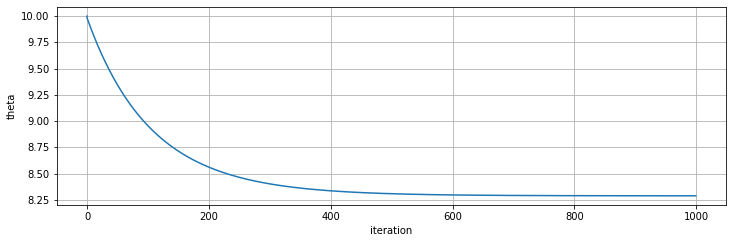
\includegraphics[width=0.9\linewidth]{index.png}

\section{Excercise 2.6}

\textbf{Theorem 2.3} Fix $T$ and let $G:\mathbb{R}^{d}\rightarrow\mathbb{R}^{d}$ be a Lipschitz-continious function. Consider the (biased version) of recursion (2.8) up to the $T$.

$$\theta_{n+1}=\theta_{n} + \epsilon(G(\theta_{n}) + \beta_{\epsilon}(\theta_{n})), n\epsilon\leq T$$

with constant step size $\epsilon > 0$. 

Let $x_{\epsilon}=\vartheta^{\epsilon}(t)$, $0 \leq t \leq T$ denote the interpolation process of $\{\theta_{n}\}$ on $[0, T]$, for $T>0$ with $x_{\epsilon}(0)=\theta_{0}$.

If $\sup_{\theta}\lVert\beta_{\epsilon}(\theta)\rVert=\mathcal{O}(\epsilon)$, the the $\epsilon$-indexed sequence of process ${x_{\epsilon}((t); 0 \leq t \leq T: \epsilon > 0}$ converges as $\epsilon \rightarrow 0$ in the sup norm) to the solution of the ODE:

$$\frac{dx(t)}{dt} = G(x(t)), 0\leq t \leq T$$

$$\theta_{n+1} = \theta_{n} - \epsilon J^{'}(\theta_{n})$$

\subsection{a)}
Show that as $\epsilon\rightarrow 0$ the interpolation process converges to the ODE:

$$\frac{dx(t)}{dt}=\frac{\sin(\alpha_{2}(x(t))}{v_{2}} - \frac{\sin(\alpha_{1}(x(t)))}{v_{1}}$$

$$G(x(t)) = \frac{\sin(\alpha_{2}(\theta))}{v_{2}} - \frac{\sin(\alpha_{1}x(t))}{v_{1}} = -\frac{1}{v_{1}}\cdot \sin(\alpha(\theta))+\frac{1}{v_2}\cdot \sin(\alpha_{2}(\theta))$$

$$G' = \frac{dG(x(t))}{dt} = -\frac{d\alpha_{1}(\theta)}{dt}\cdot \frac{\cos(\alpha_{1}(\theta))}{v_{1}} + \frac{d\alpha_{2}(\theta)}{dt}\cdot\frac{\cos(\alpha_{2}(\theta))}{v_{2}}$$

to apply theorem 2.3 we need to prove that $G(x(t))$ is Lipschitz function; then we can apply 2.3 and prove the convergence ad $\epsilon\arrow 0$. 

U\sing the mean value theorem: if $G$ is continuous in closed interval $[a, b]$ and differentiable on the open $(a, b)$ then $\exists c\in (a, b)$ such that $G'(c)=\frac{G(b)-G(a)}{b-a}$ so:

$$\lVert G(b) - G(a) \rVert = |G'(c)|\cdot \lVert b - a \rVert$$ is the case $G'(x)$ is bounded in $(a, b)$. Then we will have

$$\lVert G(b) - G(a) \rVert \geq L\lVert b - a \rVert$$

which means that $G$ is Lipschitz function.


Let $$G(x(t)) = \frac{dx(t)}{dt} = \frac{\sin(\alpha_{2}(x(t))}{v_{2}} - \frac{\sin(\alpha_{1}(x(t))}{v_1}$$

$$\Rightarrow$$

$G'(x(t)) = \frac{d\alpha_{2}(\theta)}{dt}\cdot\frac{\cos(\alpha_{2}(\theta)}{v_{2}} - \frac{d(\alpha_{1}(\theta))}{dt}\cdot\frac{\cos(\alpha_{1}(\theta))}{v_1}$$

Refer to the book page 16:

$$tan(\alpha_{1}(\theta))=\frac{\theta}{a}$$

$$tan(\alpha_{2}(\theta)) = \frac{d-\theta}{b}$$

\begin{equation}
\cos^{2}(\alpha_{1}(\theta)) = \frac{\alpha_{1}(\theta)}{d\theta} = \frac{1}{\theta}\sin(\alpha_{1}(\theta))\cos(\alpha_{1}(\theta)) =  -\frac{1}{tan(\alpha_{1}(\theta))}\sin(\alpha_{1}(\theta))\cos(\alpha_{1}(\theta))=\cos^{2}(\alpha(\theta))
\end{equation}

$$\frac{d\alpha_{2}(\theta)}{d\theta} = -\frac{1}{d-\theta}\sin(\alpha_{2}(\theta))\cos(\alpha_{2}(\theta)) = -\frac{1}{tan(\alpha_{2}(\theta))}\sin(\alpha_{2}(\theta))\cos(\alpha_{2}(\theta))$$

\begin{equation}
\frac{d\alpha_{2}(\theta)}{d\theta} = -\cos^{2}(\alpha_{2}(\theta))
\end{equation}

substitute \textbf{1} and \textbf{2}:

$$G'(x(t)) = -\frac{d\alpha_1(\theta)}{dt}\cdot\frac{\cos(\alpha_{1}(\theta)}{v_1} + \frac{d\alpha_{2}(\theta)}{dt}\cdot\frac{\cos\alpha_2(\theta)}{v_2} = \cos^{2}(\alpha_{1}(\theta))\cdot\frac{\cos(\alpha_{1}(\theta)}{v_1} - \cos^{2}(\alpha_{2}(\theta))\cdot\frac{\cos(\alpha_{2}(\theta))}{v_2}$$



$G'(x(t)) = \frac{\cos^{3}(\alpha_{1}(\theta))}{v_{1}} - \frac{\cos^{3}(\alpha_{2}(\theta))}{v_{2}} \leq \lvert \frac{\cos^{3}(\alpha_{1}(\theta)}{v1} \rvert + \lvert\frac{\cos^{3}(\alpha_{2}(\theta))}{v_{2}}\rvert \leq \lvert\frac{1}{v_1}\rvert + \lvert \frac{1}{v_2}\rvert$

Let $L = \lvert\frac{1}{v_1}\rvert + \lvert\frac{1}{v_2}\rvert$

then $G'(x(t))$ is bounded by $L = \lvert\frac{1}{v_1}\rvert + \lvert\frac{1}{v_2}\rvert$ \since $G(x(t))$ is continious and differentiable, then $G(x(t))$ is Lipschitz. Applyting theorem 2.3 to $G(x(t))$ then as $\epsilon \rightarrow 0$ the interpolation process converge to the ODE.

\subsection{b)}

Show that $\theta^{*}$ is stable and argue that a solution $x(t)$ of the above $ODE$ must then satisfy $\lim_{t\rightarrow\infty}x(t)=\theta^{*}$

$$G(x(t))=\frac{\sin(\alpha_{2}(\theta))}{v_{2}}-\frac{\sin(\alpha_{1}(\theta)}{v_{1}}$$

$$G(x(t)) = -\frac{\sin(\alpha_{1}(\theta))}{v_{1}} + \frac{\alpha_{2}(\theta)}{v_{2}}$$

constant $v_{2} < v_{1}$ then:

$$G(x(t)) \leq \lvert -\frac{\sin(\alpha_{1}(\theta))}{v_{2}}\rvert + \lvert\frac{\sin(\alpha_{2}(\theta))}{v_{2}}\rvert$$

$$G(x(t)) \leq \frac{2}{v_{2}} \Rightarrow G(x(t))$$ is bounded we can apply theorem 2.6. 

Any accumulation point $\theta^{*}$ is an asymptotically stable point $\theta^{*}$ is an asymptotically stable point of $G(x(t))$ so then $G(\theta^{*})=0$ then $\lim_{t\rightarrow\infty}(x(t))=\theta^{*}$

\end{document}
